\chapter{Implementation}

The implementation of the design of this application followed an iterative methodology, with builds moving slowly towards the design that has been described in the previous chapter. This chapter will break the application's development into distinct iterations, with the initial iteration being what was considered the Minimum Viable Product - that being that the software had fulfilled the essential requirements and its core functionality had been implemented. Each iteration will include a subsection, that defines what was included in the design at that point. The final iteration will have included all facets of the design.

\section{Iteration I: Minimum Viable Product}
\subsection{Design}
The Minimum Viable Product for the purposes of this project was defined to be the successful completion of user stories 1 and 3 (see Appendix A). In this iteration, a user interface which includes a map, that has markers on it, is created, and the markers are able to be clicked on to show their name and their description. Two forms are also created in this iteration; one form to add a point of interest, and another to edit a given point of interest. Notably, no authentication or geocoding was present in this iteration, with any user being given the ability to add or edit a point of interest.

At this stage, data and backend layers for user authentication had not been implemented. The application consisted of two views - one view containing the homepage, and the other containing a form for adding and editing a point of interest. However, all elements of the technology stack were used to implement this iteration.
\newpage

\subsection{Discussion}

\subsubsection{Google Maps for JavaScript API}

The main part of this iteration was the implementation of the Google Maps for JavaScript API, and research into how this needs to be implemented. Google provides a large set of documentation detailing possible uses for the API, as well as a tutorial on how to use it.

One important part of the implementation of the API involves the use of an API key, for authentication. This API key is linked to an account holder, with any deductions over the monthly limit being automatically invoiced to the account holder on a monthly basis by Google. The issues caused by using a Google Cloud API key are, first and foremost, the lack of the ability to transfer the API key to a customer's account, as well as the complexity of the Google Cloud interface. There are many ways in which an account holder, who may have not used cloud-based deployment platforms before, could accidentally make large purchases. Powerful 'one-click' virtual machines can be deployed in a matter of seconds, but can be very costly if not shutdown.

To mitigate this issue, restrictions were placed on the API key, that only permitted its use for requests made through its JavaScript API, and there was no authorisation for transactions over the free monthly allowance. As discussed in section~\ref{sec:googlemaps}, there is little likelihood for requests made to the API to exceed this allowance, if used solely on this application. This also reduces the likelihood of attackers, who may have extracted the API key from the source code of the homepage, being able to carry out any meaningful damage, as the API key can be easily swapped with another account, if needs be.

The core of the API implementation consists of a callback function, \texttt{async function initMap()}, that is called asynchronously as the homepage loads. The code for this is stored in a separate file, \texttt{googlemaps.js}. The function utilises the API to instantiate a map, which is then populated with points of interest through an iterative for loop. The points of interest are found through use of JavaScript's Fetch API, an interface that allows for fetching of resources. An API call is made to a method which returns all points of interest that are currently in the database.

A problem faced when implementing this part of the application was the element of difficult whilst debugging parts of the JavaScript. Google Chrome and Mozilla Firefox's debugging tools were used, however it was often difficult to pinpoint the exact issue, due to the inability to debug the function calls from Google's API. Ensuring that the click listener was correctly appended to each marker also required some prior readings into utilising JavaScript for this. Ensuring that the code was clean was also a challenge during the refactoring, with attempts made to stop code leakage and ensure the procedural programming that was being used throughout the JavaScript element of this project remained.

\subsubsection{Backend}

The backend of the application retained the simple database layer at this iteration - an un-normalised table of points of interest. In order to ensure it interfaced correctly with the database, Java Persistence API annotations had to be used. \texttt{@Entity} is an example of annotation used on \texttt{PointOfInterest}, that declares the object as an entity that has an identical relation in the database. Spring's configuration properties also had to be edited, to ensure the database that had been manually created is not dropped and replaced with Hibernate's impression of the database. However, constraints were also added directly to the object, via JPA annotations. One example is the \texttt{double latitude} member of the class. Two constraints were added to it, \texttt{@Min(value = -90, message = "Error: Latitude cannot be lower than -90")}, and \texttt{@Max(value = 90, message = "Error: Latitude cannot be greater than 90")}. These provide minimum and maximum constraints, and can pass a message if an exception is thrown, that can be shown at the view layer.

The class had to be implemented in such a way as it could be easily consumed by the data layer, without having to manually call the object's setters and passing each attribute of the form as a single attribute. The JPA allows for automatic setting of class members through either a constructor or setters. In this iteration, a constructor was used. However, setters and getters had also been created to improve the functionality of the code and assist in getting private members in other parts of the application; a unit test, for example.

In this iteration, the controller layer of the application interfaced directly with the database, as opposed to using the service layer to encapsulate the logic of the application. The application was relatively simple at the time, so it was decided that it wouldn't be necessary for an MVP to include that layer, as it would essentially be repeating repository methods without any further work carried out to the object. Spring's \texttt{@RestController} annotation, that provides controller functionality without methods being required to return a view, allowed for a RESTful API to be created without much more configuration than would be required if a standard controller was made. At that point, a \texttt{PageController}, carrying the \texttt{@Controller} annotation, had also been created to permit navigation between simple parts of the app, that did not require a model to be attached to it - the homepage, for example. In this iteration, the RESTful API created a method to list all points of interest, through utilising the \texttt{findAll()} method in JPA repositories, and add a point of interest to the database.

Difficulties were faced with creating a distinction between adding a point of interest and updating a point of interest. The \texttt{save()} method in JPA repositories will perform an SQL UPDATE, as opposed to an SQL INSERT, operation, if the primary key of the given object matches that of one object in the database. Relying on this, however, seemed to result in a conflict exception. A workaround was implemented - a second, distinct, update method and API mapping was created. This took two arguments, the Point of Interest with its updated members, and the ID of the point of interest. The ID would then have to be set within the method to allow for the SQL UPDATE operation to be triggered - with the conclusion being that the ID of any point of interest is lost within its transmission from the view layer to the controller layer.

\subsubsection{Frontend}

A number of challenges were posed when scripting the frontend of the application, including following Materialize's standards for layout development, and utilising Thymeleaf correctly and efficiently.

Thymeleaf's implementation in Spring focuses on a ``resources" folder, with two subfolders, ``static" and ``template". The first folder, as the name suggests, contains static resources - resources that Thymeleaf and Spring would not change at compile time. This included \texttt{materialize.css}, the CSS file that provides implementation of each Materialize UI components, with the JavaScript containing Materialize's JavaScript helper functions, the Google Maps function discussed above, as well as a third-party algorithm, ``lazysizes"\cite{lazysizes}. This implements the lazy-loading algorithm on images that are assigned this class; the algorithm ensuring that the resource attached to it is only loaded when required. In this instance, the algorithm was applied to images in the marker popup, to ensure they were not loaded before required, which would impact initial page load times.

The second folder contains the HTML for pages that are to be rendered onto the browser. Thymeleaf expects HTMl to be typed declaratively, as opposed to approaches frameworks such as React take. A feature of Thymeleaf, that was researched and used during this iteration, is its fragments feature. This feature allows you to place reused code into its own file, and called at the position that it would be written in a static HTML website. For example, calls to files such as Material Icons were placed in \texttt{fragments/header.html}, and, in the \texttt{<head>} tags of all templates, it was called with the line \texttt{<fragment th:replace
=\"fragments/header :: header\"></fragment>}. When this was rendered in the browser, the source would show what was in the fragment. This allowed for less reused code, and easier navigability within the resources files.

Correct placement of the map seemed to pose an issue when creating the homepage. The container for the Maps JavaScript appeared to overflow the page's default view height, requiring a user to scroll down to be able to view it. This was not a reasonable expectation for the user, particularly as it was intended to be used in a web browser set to full-screen. A workaround for this was implemented, by creating a custom CSS file. This CSS file overrode Materialize's grid system by having the height be declared manually, with the line being \texttt{height: calc(99vh - 56px);}. The height of the menu bar, at the top of the screen, measured at fifty-six pixels, according to the CSS file. With a view height of 100 still appearing to overflow the page, decrementing this by one appeared to resolve the issue, and showed an aesthetically pleasing home screen.

The `admin panel', at this stage, were two forms, one to add a point of interest, and one to edit a point of interest. Research had to take place in how to correctly manage a POST request within an HTML form when using Thymeleaf. The Thymeleaf XML namespace allowed you to call the backend from the view. Therefore, in the 'add' form, Thymeleaf calls the HTTP POST method in the controller, and instantiates an empty POI with \texttt{th:object="\$\{pointOfInterest\}"}. Each field within the HTML form also included a Thymeleaf attribute, \texttt{th:field}, that included the member of the POI object that the field relates to. This was similar in the edit form, with a duplicate form being used that is instead populated with members from the point of interest provided in the model of the view.
\newpage
\begin{figure}[!ht]
	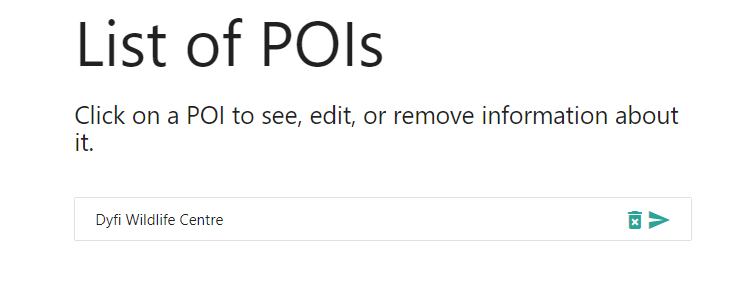
\includegraphics[scale=0.6]{diagrams/listPOI}
	\caption{An example of a point of interest list in the view layer.}
\end{figure}	


A list of points of interests also had to be made, which included edit and delete buttons for every point of interest. This was created through performing iteration within Thymeleaf, with a method call to the GET request that returns all points of interest in the database. This is called within a list object in the view as \texttt{th:each="poi : \${pointsOfInterest}"}, and is populated at runtime, with the rendered view containing every point of interest. This allows for simplicity to be achieved in the view, and negates the need for JavaScript, as an example, to be used, reducing the amount of code within one view.
% 1995 words
% Total: 8562 words
% Remaining: 3438 words

\section{Iteration II: Admin authentication}
\subsection{Design}

\subsection{Discussion}

\section{Iteration III: Geocoding}
\subsection{Design}

\subsection{Discussion}

\section{Iteration IV: Map additions and final build}

\subsection{Design}

\subsection{Discussion}
